\documentclass[10pt, english]{article}
\usepackage[top=3.6cm, bottom=3.6cm, left=1.75cm, right=1.75cm]{geometry}
\geometry{a4paper}
\usepackage[T1]{fontenc}
\usepackage[utf8,latin1]{inputenc}
\usepackage[english]{babel}
\usepackage{layout}
\usepackage{titlesec}
\usepackage{lastpage}
\usepackage{eurosym}
\usepackage{caption}
\usepackage{eurosym}
\usepackage{amsmath,amssymb} % packages pour les environnements et symboles mathématiques
\usepackage{graphicx} % packages graphique (pour inclure des images)
\usepackage{subfig}
\usepackage{float}
\usepackage{listings} % package pour lire 
\usepackage{lscape} % Package pour les paysages
\usepackage{setspace}
%%\renewcommand{\figurename}{\vspace{-10pt}\textbf{\bsc{Figure}}}
%%\renewcommand{\thefigure}{\textbf{\arabic{figure}}}
%%\renewcommand{\thesubfigure}{\textbf{(\alph{subfigure})}}

%% créer les figure en latex
\usepackage{tikz}
\usetikzlibrary{shapes.geometric, arrows}
\tikzstyle{startstop} = [rectangle, rounded corners, minimum width=3cm, minimum height=1cm,text centered, draw=black, fill=red!30]
\tikzstyle{process} = [rectangle, minimum width=3cm, minimum height=1cm, text centered, draw=black, fill=orange!30]
\tikzstyle{arrow} = [thick,->,>=stealth]
%%


\topmargin=0pt
\headheight=0pt
\headsep=0pt
\marginparsep=0pt
\marginparwidth=0pt
\footskip=30pt
\marginparpush=0pt
\textheight=670pt

\titleformat*{\section}{\large \bf}
\titleformat*{\subsection}{\normalsize \bf}

\let\originalparagraph\paragraph
\renewcommand{\paragraph}[1]{\originalparagraph{#1.}}

\title{\Large{\bf{Smartee\\ Smart, Eco-friendly \& Economic Box\\ Project 2}}}

\author{
  \normalsize{Antoine BOUCHAIN} \\
 \small{\texttt{abouchain@enseirb-matmeca.fr}}
  \and
  \normalsize{Mathias DE CACQUERAY VALMENIER}\\
 \small{\texttt{mdecacquerayvalmenie@enseirb-matmeca.fr}}
    \and
    \normalsize{Melinda GOZLAN}\\
 \small{\texttt{mgozlan@enseirb-matmeca.fr}}
  \and
  \normalsize{Xavier LETURC}\\
  \small{\texttt{xleturc@enseirb-matmeca.fr}}
    \and
    \normalsize{Marc PRATS-ESCRIBANO}\\
  \small{\texttt{mpratsescribano@enseirb-matmeca.fr}}
  \and
  \normalsize{Benjamin RAMBAUD}\\
 \small{\texttt{brambaud@enseirb-matmeca.fr}}
  \and
  \normalsize{Karim TOUFIQUE}\\
  \small{\texttt{ktoufique@enseirb-matmeca.fr}}
}

\date{}

\captionsetup{labelsep=period, font=small, labelfont=bf}

\makeatletter
\renewcommand{\@oddfoot}{\hfil \thepage\ of \pageref{LastPage} \hfil}
\makeatother

\begin{document}

\maketitle

\vspace{-20pt}
\begin{center}
Supervisors:\\
\vspace{5pt}
\begin{minipage}[c]{150pt}
\begin{center}
  \normalsize{Guillaume FERR\'{E}}\\
  \small{\texttt{guillaume.ferre@ims-bordeaux.fr}}
\end{center}
\end{minipage}
\hspace{20pt}
\begin{minipage}[c]{150pt}
\begin{center}
  \normalsize{Jean-R\'{e}my FALLERI}\\
  \small{\texttt{falleri@labri.fr}}
\end{center}
\end{minipage}
\end{center}
\begin{figure}[h]
 \begin{center}
   \subfloat{
   
\includegraphics[width=0.4\textwidth]{figures/logo_ENSEIRB.pdf}
   \label{fig1}
   }
   \subfloat{
   
\includegraphics[width=0.4\textwidth]{figures/logo_SMARTEE.pdf}
   \label{fig2}
   }
 \end{center}
\end{figure}

% abstract


\vspace{10pt}

\begin{abstract}
\noindent The aim of this document is to introduce the Smart-Eco Box project. This smart-eco box is called Smartee and ot can connect to the user's sensors to help him to regulate his energy consumption. Our biggest challenge in designing the box was to display the devices engergy consumption in a website and to detect whether the sensors are on or off.
The workload was splitted between two teams: one tacking care of signal processing and the other one of the website design. The signal processing part dealt with the signal emission by the sensors, the analysis of transmitted data and the detection of the devices. We also had to design a user-friendly interface that had to display in an ergonomic and understandable manner the information retrieved thanks to the signal processing.

\end{abstract}
\vspace{10pt}


% document

%%%%%%%%%%%%%%%%%%%%%%%%%%%%%%%%%%%%%%%%%%%%%%%%%
%                                               %
%%%%        Context of the Project           %%%%
%                                               %
%%%%%%%%%%%%%%%%%%%%%%%%%%%%%%%%%%%%%%%%%%%%%%%%%
%%%%%%%%%%%%%%%%%%%%%%%%%%%%%%%%%%%%%%%%%%%%%%%%%%%%%%%%%%%%%%%%%%%%%%%%%%%%%%%%%%%%%%%%
%
%   Context of the Project
%
%%
%%%%%%%%%%%%%%%%%%%%%%%%%%%%%%%%%%%%%%%%%%%%%%%%%%%%%%%%%%%%%%%%%%%%%%%%%%%%%%%%%%%%%%
\section{Introduction}

Today mastering his domestic energy consumption is a major stake in our society. Everyear, bills related to energetic ressources increase, in 2013 French homes paid 3210\euro, an increase of more than 40\euro compared with 2012. And the ways set up to reduce them such as solar panels are still too expensive for the majority of the population and not enough effective during winter seasons.\\

In this context, the global objective of the project is to work on the design of a "box" called Smartee that can minimize the energy consumption of a building and maximize comfort. The Smart-Eco Box project was developed in a new growing market, known as Smart Energy Boxes. Although many sensors are already on the market, they are usually heterogeneous (i.e. non-standardized ) which complicates their use in a system such as the one we would like to develop. Therefore members of the project will design a wireless communication system (box + associated sensors) for intelligent and efficient supervised management of energy consumption of a building on a website including the ability of the box to identify an electrical device in its ignition.\\

Once plugged in, the Smartee initialization detects sensors in the environment. Then a processing phase allows the box to work without any need for input by the client. This software allowed to detect bursts and initiated bursts processing received by a provided Universal Software Radio Peripheral (USRP). Finally data are stored in a database and energy consumption of the place is displayed on the website.

\subsection{Context}

%Dans un monde de plus en plus connecté et soucieux de l’environnement, nos maisons se transforment en habitats intelligents, et permettent notamment une meilleure gestion des dépenses énergétiques au quotidien. Ces dernières années, de nombreux systèmes de domotique assurant la gestion des équipements (portails, volets, lumières) sont arrivés sur le marché. Néanmoins, très peu de ces systèmes permettent le suivi détaillé et le pilotage énergétique de l’ensemble des équipements au sein de l’habitat. Période de crise et diminution du pouvoir d’achat poussent les Français à réaliser des économies dans tous les domaines. Selon l’ADEME (Agence de l’environnement et de la maîtrise de l’énergie), la facture moyenne (toutes énergies confondues) s’est élevée en 2012 à 1 403 euros par ménage, contre 1 239 euros en 2007. Aujourd’hui, 80\% des ménages cherchent à réduire leur consommation d’énergie, notamment via des comportements plus économes en terme d’éclairage et de chauffage. Un nouveau secteur est en train de naître, les smart energy boxes. Certains fabricants du domaine énergétique tels que Legrand ou Schneider Electric proposent déjà des solutions comme les premiers compteurs électriques connectés. Le projet Ecobox s’inscrit dans une démarche de meilleure gestion de l’énergie par un pilotage autonome et automatisée de l’habitat.

\subsection{Smart EcoBox Description}
% Quel est le but de la box ?
%
% déroulement du process : recevoir trame, décoder, inserer dans db. detection des états des appareils. affichage des infos sur le client.
%
% pourquoi avoir choisi Raspberry Pi ?
%   box doit être petite (cad pas un gros pc etc..)
%   peu cher -> correspond au souhait du client d'avoir une box abordable
%   comme ça a peu de ressources, si ça passe dessus peu importe les ressources dispo dans le future


The \textbf{Smart EcoBox} project is aimed to help people manage their energy consumption and therefore enabled a reduction of their energy bills.

%La gestion des équipements de la maison par l’intermédiaire de terminaux tels que tablettes ou téléphones permettra de simplifier la vie de l’utilisateur au quotidien.

\begin{figure}[H]
\centering
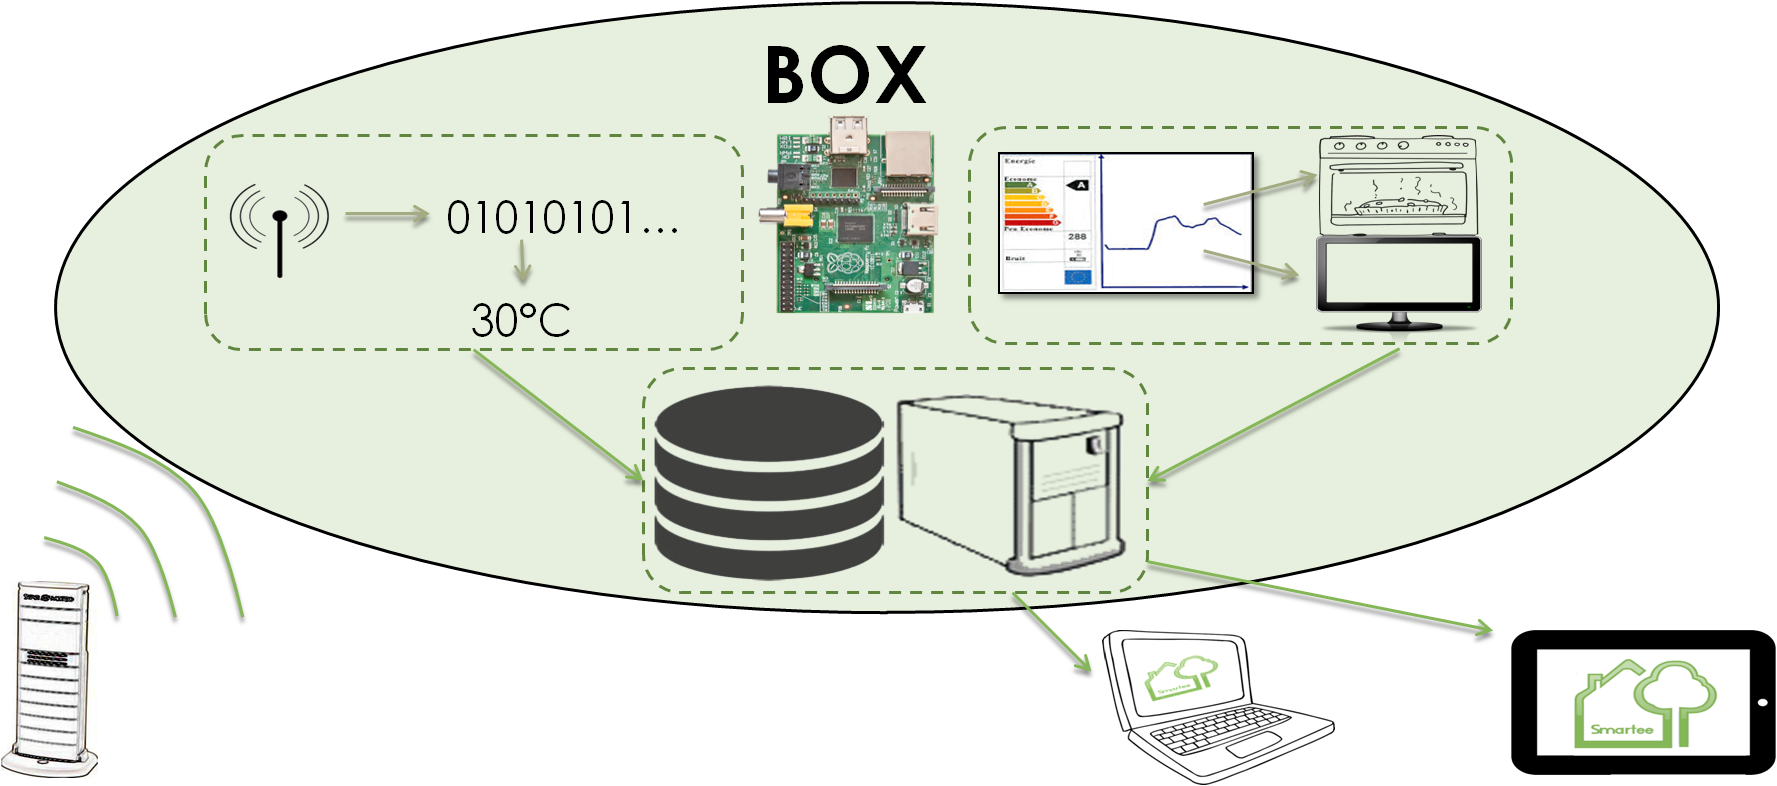
\includegraphics[scale=0.4]{figures/box.png}
\caption{Smart Eco Box Description}
\label{fig:boxDescription}
\end{figure}


%%%%%%%%%%%%%%%%%%%%%%%%%%%%%%%%%%%%%%%%%%%%%%%%%
%                                               %
%%%%        Research                         %%%%
%                                               %
%%%%%%%%%%%%%%%%%%%%%%%%%%%%%%%%%%%%%%%%%%%%%%%%%
%%%%%%%%%%%%%%%%%%%%%%%%%%%%%%%%%%%%%%%%%%%%%%%%%%%%%%%%%%%%%%%%%%%%%%%%%%%%%%%%%%%%%%%
%
%   Research                   
%
%%
%%%%%%%%%%%%%%%%%%%%%%%%%%%%%%%%%%%%%%%%%%%%%%%%%%%%%%%%%%%%%%%%%%%%%%%%%%%%%%%%%%%%%
\section{Research}

The strength of our device lies in its ability to determine precisely which device is turned on or not. Thankfully, each device has a specific load curve, and analyzing different points of the load curve helps to determine when a device turns on. Two different approaches were proceeded, a macroscopic and a microscopic one. The main difference between them are the sampling frequency and the focused points of the curves. The macroscopic approach requires about 1Hz and studies the whole form of the load curve whereas, for the microscopic one, it requires between 5 and 10 kHz and studies the transient response.

%%%%%%%%%%%%%%%%%%%%%%%%%%%%%%%%%%%%%%%%%%%%%%%%%
%       Macroscopic analysis of load curve      %
%%%%%%%%%%%%%%%%%%%%%%%%%%%%%%%%%%%%%%%%%%%%%%%%%
%%%%%%%%%%%%%%%%%%%%%%%%%%%%%%%%%%%%%%%%%%%%%%%%%
%       Macroscopic analysis of load curve      %
%   Antoine                                     %
%%%%%%%%%%%%%%%%%%%%%%%%%%%%%%%%%%%%%%%%%%%%%%%%%
\subsection{Macroscopic Analysis of a Load Curve}
A fast algorithm is needed and that can be called at any moment to detect a device. It is based on a study of the load curve. In case the results of this approach are doubtful, the microscopic algorithms are used.

The following approach comes from the work achieved by Mr. El Guedri \cite{research1}. The macroscopic algorithms are based on the differentiate function, which helps detect a jump in the load curve. Indeed the difference between two points of a jump is directly the consumption of the device, as shown in \ref{fig1} where the grouped squares are a heater use.


\begin{figure}[h]
 \begin{center}
   \subfloat[Example of a real load curve]{
   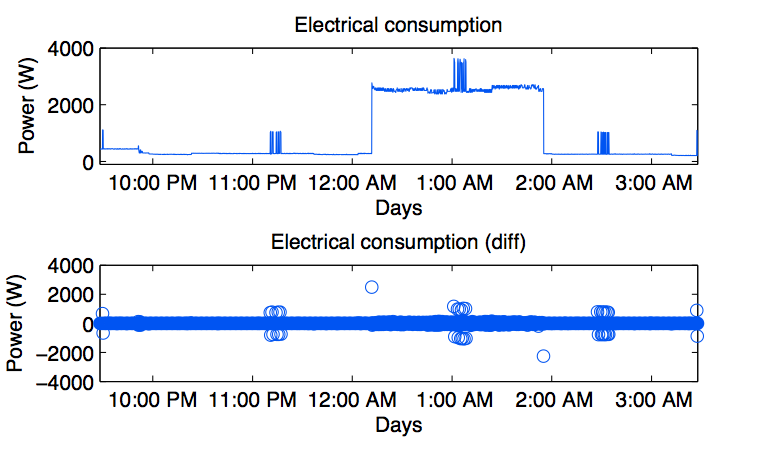
\includegraphics[width=0.45\textwidth]{figures/fig_antoine_5.png}
   \label{fig1}
   }
   \subfloat[Estimation of a heater consumption]{
   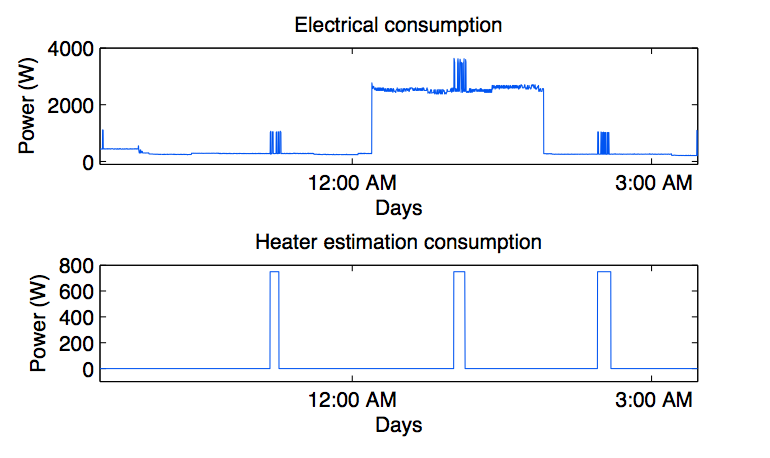
\includegraphics[width=0.45\textwidth]{figures/fig_antoine_6.png}
   \label{fig2}
   }
   \caption{Macroscopic Analysis}
   \label{fig-1-1-2}
 \end{center}
\end{figure}

Several steps of consumption were defined: $100$, $500$ and $750W$ which mean small consumption device (such as lights), medium consumption (oven) and heavy consumption (heater). The load curve reaching one of these values means the device is turning on, and reaching the same negative value means the device is turning off. With this basic approach some devices can be defined, but it is not possible to differentiate an unknown device consuming 500W from an oven for example.

Therefore, a second algorithm was developed that analyzes the signature load curve of each device. Every device has a specific and unique load curve when they turn on. If a data base were created with these signatures, they could be used to determine which device has just turned on. Spotting when the devices turn off is simple as it corresponds to negative values of the differentiate function.

An example will help make the description clearer. A heater power consumption load curve is basically a square repetition. This shape is due to the periodicity of the device. By detecting such a wave form in the load curve, then we can detect heater consumption and estimate the consumption of this device. These results are shown on the figure \ref{fig2}.


Non periodical devices are processed in the same way, such as a dishwasher or a washing machine. But at the moment, only the dishwasher has been implemented.

% Transition
% As the sampling frequency is quite low, to devices


%%%%%%%%%%%%%%%%%%%%%%%%%%%%%%%%%%%%%%%%%%%%%%%%%
%       Microscopic analysis of load curve      %
%%%%%%%%%%%%%%%%%%%%%%%%%%%%%%%%%%%%%%%%%%%%%%%%%
%%%%%%%%%%%%%%%%%%%%%%%%%%%%%%%%%%%%%%%%%%%%%%%%%
%       Microscopic analysis of load curve      %
%   Xavier                                      %
%%%%%%%%%%%%%%%%%%%%%%%%%%%%%%%%%%%%%%%%%%%%%%%%%

\subsection{Microscopic analysis of the load curve}
%Xavier
The sampling frequency used in the case of a microscopic analysis of the load curve is between 5 and 10k$Hz$. Such a frequency is required to access the transient responses of the devices. Using such a high sampling frequency is a way to avoid a difficulty encountered in macroscopic analysis coming from the fact that an appliance is generally switched on while other appliances are already in use. 
\\

An important point is that the transient response is linked with the physical role of the device. Studies have then been conducted to isolate characteristic parameters of the appliance from the transient response. Here is an example of a transient response :
\\
% Figure

\begin{figure}[H]
\centering
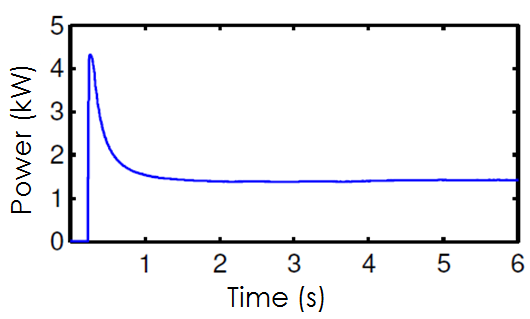
\includegraphics[scale=0.5]{figures/transient_response.png}
\caption{Transient response}
\label{fig:transient_response}
\end{figure}


[2] address the problem of classification of transient signals which are modelled as a Smooth transition autoregressive model. Figure x shows some abrupt transitions on the transient signal, which are called breakpoints. Let $K$ denote the number of breakpoints, and $\underline{\tau} = [\tau_1,...,\tau_K]$ denote the sequence of the $K$ breakpoints. By convention, $[\tau_0;\tau_{K+1}]$ represents the observation interval of the signal. 
\\

 Therefore, the signal is modelled as a linear combination of regression functions $\{m_k\}_{k\in{1,K+1}}$.~$m_k$ is the regression model of the signal over the segment $[\tau_{k-1};\tau_{k}]$. Then, the signal is expressed as

\begin{equation}
\forall t\in [\tau_0;\tau_{K+1}],m(t)= \sum_{k=1}^{K+1}p_k(t)m_k(t)
\end{equation}

where $p_k(t)$ is the weight function of the $k^{th}$ regression model which can be expressed as follow
\begin{equation}
\forall k\in [1,K+1], p_k(t)= \pi_{\eta_{k-1}}(t-\tau_{k-1})-\pi_{\eta_{k}}(t-\tau_{k})
\end{equation}

$\pi_{\eta_{k}}$ is the transition function of the $k^{th}$ breakpoint, which depends on a vector of parameter $\eta_{k}$. In the model described in [1], $\pi_{\eta_{k}}$ is a sigmoide function, whose expression is 
\begin{equation}
\pi_{\eta_{k}} = \frac{1}{1+exp(\frac{t}{\lambda_k})}
\end{equation}

The only element in $\eta_{k}$ is then $\lambda_k$, which is a scale parameter. Let $\underline{\lambda}$ denote the concatenation of all the scale parameters $\underline{\lambda} = [\lambda_1,...,\lambda_K]$.
\\

 Regression model are considered in [2] as polynomial 

\begin{equation}
m_k(t)= \sum_{q=0}^{Q_k} \beta^{(q)} _kt^q
\end{equation}

$\beta^{(q)} _k$ is the $q^{th}$ order regression coefficient of the $k^{th}$ regression model, and $Q_k$ is the order of $m_k(t)$. As it was the case for $\lambda$, $\beta$ regroups all the $\beta_k$ coefficients and $Q$ all the $Q_k$ coefficients.
\\

A common model for the observed signal is 


\begin{equation}
s(t)=m(t) + \epsilon (t)
\end{equation}

$\epsilon (t)$ is an additive white Gaussian noise whose variance is $\sigma^2$. The different parameters which have to be evaluated are then :
\begin{equation}
\theta=\{\underline{\lambda},\underline{\tau},\underline{\beta},\underline{Q},\sigma ^2,K\}
\end{equation}
\\


The approach presented in [2] is a Bayesian one. The $posterior$ probability density function of $\theta$ is obtained thanks to the Bayes formula. The algorithm used to sample the distibution is a Reversible Jump Markov chain Monte Carlo (RJMCMC). The algorithm consists in a main loop which is repeated a high number of time. The higher the number of iterations, the more accurate the algorithm. A new set of values is purposed for $\theta$ during each iteration. The different kind of movements that can be purposed concerning $\theta$ are :
\begin{itemize}
\item Birth of a transition
\item Death of a transition
\item Division of an existing transition
\item Fusion of two existings transitions
\item Update of a transition
\end{itemize}
The movement is then accepted or rejected with a certain probability, which depends on Hasting-Green-Metropolis ratio. 
\\

The classification of electrical devices is then done thanks to $\theta$. Since that study was more a theoretical than a practical work, it has not been implemented yet on the box, but is functionnal for very basics signals.




%%%%%%%%%%%%%%%%%%%%%%%%%%%%%%%%%%%%%%%%%%%%%%%%%
%                                               %
%%%%        Signal Processing Algorithm      %%%%
%                                               %
%%%%%%%%%%%%%%%%%%%%%%%%%%%%%%%%%%%%%%%%%%%%%%%%%
%\section{Signal Processing Algorithm}
%%%%%%%%%%%%%%%%%%%%%%%%%%%%%%%%%%%%%%%%%%%%%%%%%%%%%%%%%%%%%%%%%%%%%%%%%%%%%%%%%%%%%%%%
%
%   Signal Processing Algorithm                  
%
%%
%%%%%%%%%%%%%%%%%%%%%%%%%%%%%%%%%%%%%%%%%%%%%%%%%%%%%%%%%%%%%%%%%%%%%%%%%%%%%%%%%%%%%
\section{Sensors Data Processing}
Our box needs information of Temperature, Electric consumption... All this data are easily retrieved from sensors already in the market. For this project two sensors had been chosen : the Electric consumption Chacon's Ecowatt 850 and the DIO TX-35 for temperature. Both those sensors send information at a rate of one samples every two seconds.\\
This sensors use the IHM band at 433 MHz. The particularity of this band is that it is completely free of use. There is no communication rules, hence, each constructor, each sensor use a different way to communicate. Both sensors are using 2-FSK modulation : 2 frequency shift keying modulation. \\
On this job, two people were assigned at first, they principal work was to understand and enhance code already produce in \textsc{C++} last year. Eventually, all the reception chain was rewritten for low consumption. Improvement is describe in the next section.
\subsection{Burst Retrievement}
Originally, signal with information was separated from noise on a per sample basis. It was a comparison between the lowest value of instantaneous power and each sample value. It is not a correct approach, because power should be calculated on multiple samples.\\
To enhance this part, and reduce consumption, we started working on average power on 4096 samples. Result were enhance using this technique, also it reduce power consumption, because comparison is done only every 4096 samples.
\subsection{Demodulation}
Last year, modulation and demodulation were automated, it is not needed anymore. Because of the presence of only two sensors, which both are using 2-FSK modulation.
\subsection{MAC information decoding}
After the signal is demodulated, it is possible to know from which sensor the information is coming. Number of bits is usually used.
From observations it is possible to reverse engineer the sensor coding solution. It is always different, and not logical. For instance, in the EcoWatt sensor, it was determine than a "1" bit was coded by \texttt{110} and a zero bit by \texttt{111}. Also how is coded the main information : consumption or temperature is not trivial. Linear regression are used to determine which bits are coding it, and how.
\subsection{Database Sending}
When all those operations are done, a timestamp with the unique ID and the data of the sensor is sended to the database.

%%%%%%%%%%%%%%%%%%%%%%%%%%%%%%%%%%%%%%%%%%%%%%%%%
%                                               %
%%%%        Web application                  %%%%
%                                               %
%%%%%%%%%%%%%%%%%%%%%%%%%%%%%%%%%%%%%%%%%%%%%%%%%
%%%%%%%%%%%%%%%%%%%%%%%%%%%%%%%%%%%%%%%%%%%%%%%%%%%%%%%%%%%%%%%%%%%%%%%%%%%%%%%%%%%%%%%
%
%   Web application                   
%
%%
%%%%%%%%%%%%%%%%%%%%%%%%%%%%%%%%%%%%%%%%%%%%%%%%%%%%%%%%%%%%%%%%%%%%%%%%%%%%%%%%%%%%%
\section{Web application}

%%%%\subsection{Server}
%%%%%%%%%%%%%%%%%%%%%%%%%%%%%%%%%%%%%%%%%%%%%%%%%
%       Server                                  %
%                                               %
%%%%%%%%%%%%%%%%%%%%%%%%%%%%%%%%%%%%%%%%%%%%%%%%%
\subsection{Server \& Database}

% doit tourner sur Raspberry Pi 
%   -> serveur léger -> lighttpd
%   -> db -> sqlite
%
%   php
%   ¿ interface C/C++ pour le signal ?
%%
%%%
%%
%
% la partie Serveur Web + Base de données étant deployée sur la rasberrypi qui a peu de ressources, les technos utilisées dans cette partie doivent consommer peu de ressources d'où le choix de SQLite et Lighttpd
%
% Ensuite faut dire en quoi SQLITE et Lighttpd sont légers, par exemple SQLite fonctionne sans serveur mais juste en lecture écriture de fichiers, et chercher pour lighttpd des arguments aussi.
%
% Ensuite vu que le serveur ne fait que servir les données, il faut que toute la génération des vues se fasse du coté client d'où le choix d'AngularJS ...

The web server and the database are the links between the signal processing algorithms and the web application. For this project, they are deployed on the single-board computer \textit{Raspberry Pi}. Since it has low ressources, the technologies used for the server and the database have to consume few resources. That is why SQLite and Lighttpd were chosen respectively for the database and the server.

\subsubsection{Database}

    % en quoi sqlite est léger
    %   http://www.sqlite.org/limits.html
    %   http://sqlite.org/mostdeployed.html
    % simplicité : il n'y a aucune manipulation à faire, le fichier sqlite est créé automatiquement à la volée, toute la base est stockée dans un fichier unique qu'il est facile d'échanger. 
    % http://en.wikipedia.org/wiki/SQLite
    \paragraph{SQLite Database}
    
    SQLite is a standalone relational database management system. In contrast to other database management systems, it is not implemented as a separate process that a client program running in another process accesses. Rather, it is part of the using program. SQLite is a popular choice as embedded database for local/client storage in application software such as web browsers. It is one of the most widely deployed database engine, as it is used today by several widespread browsers, operating systems, and embedded systems, among others. 
    
    
    % Structure de la base
    % description des tables etc..
    \paragraph{Structure}
    
    This paragraph introduces the different tables of the database. It has been built to be easily reshaped depending on the research results, and also to deal with big data issues. % ce n'est pas vraiment big data...
    
    \begin{itemize} % ¿ lists ou manage ?
    \item Sensors identification: lists all sensors connected to the system
    \item Locations: lists all sensor locations
    \item Data types: lists the different data types handled by the system
    \item Sensors values: lists the different sensors values recorded over time
    \item Devices types identification: lists the different device types identificated
    \item Devices status: lists all device statuses
    \item User: lists all user information
    \end{itemize}
    
    % ajouter schéma conceptuel de la base.
    
\subsubsection{Server}

    % le serveur ne fait que servir les données
    With the chosen architecture, the web server only sends the data to the client dealing with their processing.
    
    % en quoi lightpd est léger
    % cf references de http://en.wikipedia.org/wiki/Lighttpd
    \paragraph{Lighttpd Server}
    Lighttpd is a secure, fast, compliant, and flexible web server that has been optimized for high-performance environments. It has a very low memory footprint compared to other web servers and takes care of cpu-load.








%%%%\subsection{Client}
%%%%%%%%%%%%%%%%%%%%%%%%%%%%%%%%%%%%%%%%%%%%%%%%%
%       Client                                  %
%                                               %
%%%%%%%%%%%%%%%%%%%%%%%%%%%%%%%%%%%%%%%%%%%%%%%%%
\subsection{Client} % Interface Client
\begin{figure}[H]
\centering
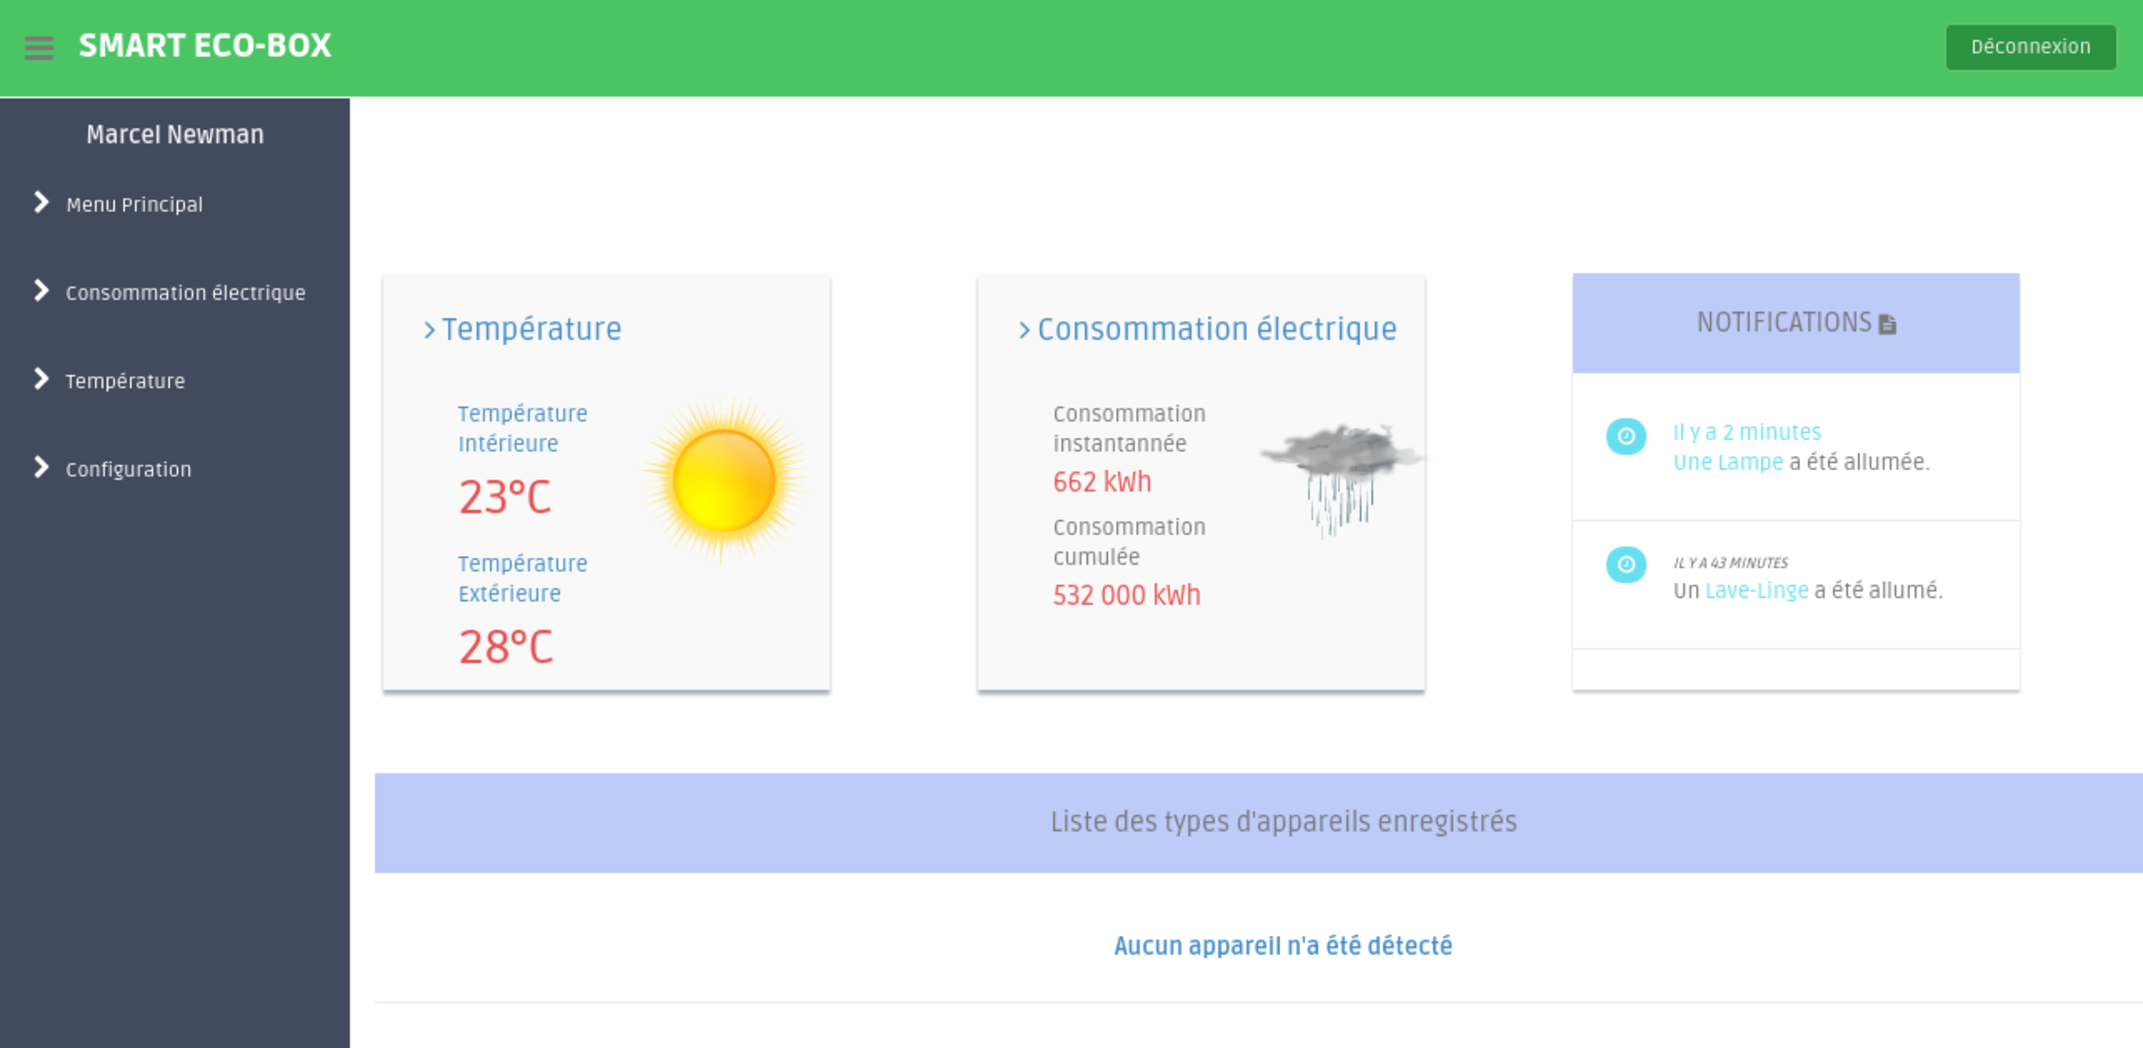
\includegraphics[scale=0.4]{figures/Accueil.pdf}
\caption{Homepage of the webapp}
\label{fig:Accueil}
\end{figure}
This subsection introduces the design of the web interface, especially the structure and the implementation of the main features.
% expliquer l'utilité de l'interface

%%%%%%%%%%%%%%%%%%%%%%%%%%%%%%%%%%%%%%%%%%%%%%%%%%%%%%%%%%%%%%%%%%%%%%%%%%%%%
\subsubsection{Structure}
    % serveur léger -> traitement côté client -> JS -> Angular
    % parler MVC avec Angular
    % n3-chart : n3-chart makes creating beautiful charts for AngularJS application easy and semantic. It is built on top of D3.js library.
    %
    % schéma du site
    Given that the server has to be light and has only to provide the data, this interface has been built with the framework AngularJS 1.3. Indeed, it enables efficient and easily maintainable client-side data processing. In addition, it is based on the Model-View-Controller architectural pattern (MVC) that allows easy maintenance of the code. The curves have been built with the n3-chart library. It makes creating charts for AngularJS application easy and semantic and it is built on top of D3.js library.
    
    The interface has four main pages reachable via the navigation bar: Homepage, Power Consumption page, Temperature page and the Configuration page. Besides, the login page to access the web app and the page to set up and configure the box are designed.
     
    \begin{figure}[!h] 
        \centering
        % pour changer la couleur
        %%  cf main.tex à \tikzstyle pour tout le document
        %   ou
        %%  cf webapp.tex pour savoir comment changer la couleur d'un node
        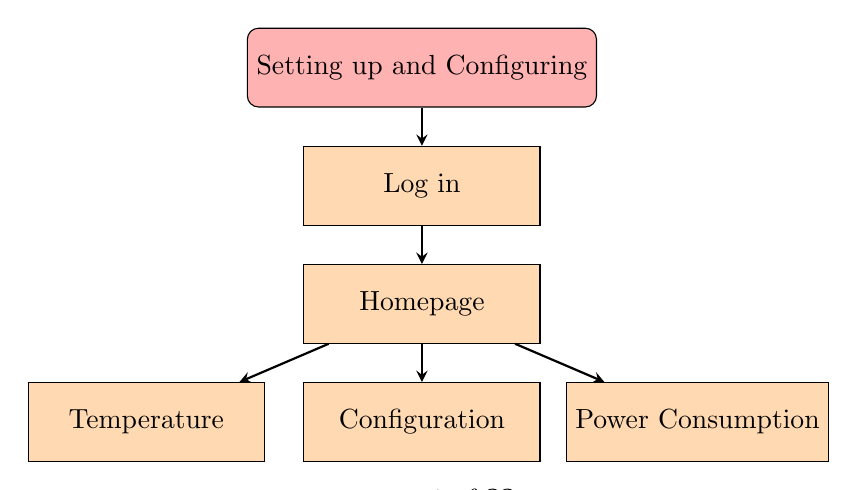
\begin{tikzpicture}[node distance=1.5cm]
    
        \node (startConf) [startstop] {Setting up and Configuring};
        \node (login) [process, below of=startConf] {Log in};
        \node (home) [process, below of=login] {Homepage};
        \node (conf) [process, below of=home] {Configuration};
        \node (conso) [process, right of=conf, xshift=2cm] {Power Consumption};
        \node (temp) [process, left of=conf, xshift=-2cm] {Temperature};

        \draw [arrow] (startConf) -- (login);
        \draw [arrow] (login) -- (home);
        \draw [arrow] (home) -- (conf);
        \draw [arrow] (home) -- (conso);
        \draw [arrow] (home) -- (temp);
        \end{tikzpicture}
    \end{figure}

     
%%%%%%%%%%%%%%%%%%%%%%%%%%%%%%%%%%%%%%%%%%%%%%%%%%%%%%%%%%%%%%%%%%%%%%%%%%%%%
\subsubsection{Homepage}

The homepage provides quick access to the general state of the system.
The main information related to the system's operation and an overview of the data sent by the sensors can be found on this page.
The homepage includes four main blocks:%, - one for electric consumption and one for temperature, one for notifications and one for the states of registered devices - where the most important data will be indicated.
    \paragraph{Power Consumption} 
    This block provides access to two types of information: the instantaneous and accumulated power consumption. An icon related to the theme of meteorology indicates the evolution of these data. % TODO Button to switch and see the cost
    \paragraph{Temperature}
    This block provides access to two main information: inside and outside temperatures.
    \paragraph{Notifications}
    This block enables the user to monitor changes of sensor statuses and registered types of device statuses. The system notifies the user when a status changes.
    %State sensor
    %State registered devices
    \paragraph{List of Devices} % Liste des types d’appareils enregistrés
    This block provides access to all registered types of devices and their statuses.
    %know the state of all registered type of devices.

%%%%%%%%%%%%%%%%%%%%%%%%%%%%%%%%%%%%%%%%%%%%%%%%%%%%%%%%%%%%%%%%%%%%%%%%%%%%%
\subsubsection{Power Consumption}

    \paragraph{Curve Page}
    % suivre evolution de sa conso
    %   courbe de conso
    %   courbe de coût associé
    %   coût cumulé sur la période.
    The user can access the evolution of his domestic power consumption thanks to three elements of information: the power consumption curve, the matched cost curve and the accumulated cost.
    
    \paragraph{Estimated Electricity Bill}
    An estimated electricity bill can be viewed on this page. It is inspired by a real electricity bill and allows the user to know an estimate depending on his behavior.
%%%%%%%%%%%%%%%%%%%%%%%%%%%%%%%%%%%%%%%%%%%%%%%%%%%%%%%%%%%%%%%%%%%%%%%%%%%%%
\subsubsection{Temperature}
    % suivre evolution de la temperature au sein sa maison
    %   courbes de temperature
    %   plusieurs capteurs
    For each temperature sensor, a temperature curve can be displayed allowing the user to access the evolution of the temperature within the house. 
%%%%%%%%%%%%%%%%%%%%%%%%%%%%%%%%%%%%%%%%%%%%%%%%%%%%%%%%%%%%%%%%%%%%%%%%%%%%%
\subsubsection{Configuration Pages}
    
    \paragraph{Setting up and Configuring} % configuration à l'allumage
    
    When the user turns on his box for the first time, he needs to register by providing his personal data: name, email, password, city and his EDF subscription. Then, the system automatically displays the different sensors detected thanks to the signal processing algorithm. The user has to set up the system by providing the name, the location and the type of each sensor. % (a color-based recognition could be used)
    
    \paragraph{Current Usage} % pendant l'utilisation
    
    \subparagraph{"My Account" Page:} 
    The user can access his personal information and change them. This includes his name, password, email, city and his EDF subscription. Similarly, the profile appears on the homepage.
    
    \subparagraph{"My Sensors" Page:}
    This page is used to list the different sensors. Each sensor can be renamed by the user, may indicate a location specified by the user (e.g. children's room) and also specifies a type of sensor that is recognized by a color code. Besides, the SNR (Signal-to-Noise Ratio) is indicated as the form of bars to show the state of a sensor (like mobile phone signal bars). Finally, users can edit the sensor information using the "Edit" button.


%%%%%%%%%%%%%%%%%%%%%%%%%%%%%%%%%%%%%%%%%%%%%%%%%
%                                               %
%%%%       Conclusion                        %%%%
%                                               %
%%%%%%%%%%%%%%%%%%%%%%%%%%%%%%%%%%%%%%%%%%%%%%%%%
%%%%%%%%%%%%%%%%%%%%%%%%%%%%%%%%%%%%%%%%%%%%%%%%%%%%%%%%%%%%%%%%%%%%%%%%%%%%%%%%%%%%%%%%
%
%   Conclusion                   
%
%%
%%%%%%%%%%%%%%%%%%%%%%%%%%%%%%%%%%%%%%%%%%%%%%%%%%%%%%%%%%%%%%%%%%%%%%%%%%%%%%%%%%%%%%
\section{Team Management}

Team Management was an important part of this project. Because it gathered people from two minors of the Telecommunication department and weekly schedules for both teams were different. Communication needed to be guaranteed throughout the project. Since the first day, tools were chosen to make it easier : the Git tool for code sharing, publishing, reviewing, testing, Azendoo website for discussion about the aspects of the project and team meeting every week to assure that no problem could raise due to communication at any step. Also, several meetings were scheduled with the client to check if our proposals were matching his expectations. Besides, in order to monitor the development, a testing version of the webapp was made available online.\\

\section{Conclusion}

To sum up, this project was a great opportunity to test team members capacity to collaborate with people of different skills. On the signal processing part, there is still work to do, the microscopic detection has just been started, while the macroscopic application can be developed with more levels and a bigger data base.

% partir du principe que l'on devait utiliser un système possèdant peu de ressource contrairement à ce qui a été fait l'année passée.
%
% db :
%   pour le moment en local sur raspberry
%   simple
%   un SGBD léger
%   tables pensées pour être maléables
%   TODO :  rajouter table Utilisateur ¿ toujours pas fait ?
%           ¿ script pour s'occuper des insert côté isnc ?
%
% server :
%   pour le moment en local sur raspberry
%   simple (ne fait qu'envoyer les données au client)
%   léger
%   TODO : ¿ rien vu qu'il ne fait rien ? 
%
% client :
%   s'occupe du traitement des data
%   dev avec maintenance et reprise de code par d'autres en tête
%   TODO : quelques pages non finis mais commencés. Fix quelques bugs par çi par là

The web application was designed to run on a low resources system contrary to previous work on Smart-Eco-Box. Indeed, the chosen database management system is light, easy to use and maintain. The database was designed to be easily reshaped depending on the research results. The chosen web server is light, compliant and simple since it only sends the data to the web client dealing with the data processing. The web interface was designed to be easily maintainable and to enable its reusability. Nevertheless, there are still unfinished webpages and unfixed bugs. Finally, the implementation of the box's intelligence started further to the research and the opportunities proposed by the web interface.



\begin{thebibliography}{10}
 \bibitem{context}
 Commissariat g\'en\'eral au d\'eveloppement durable - Service de l'observation et des statistiques, \emph{Bilan \'energ\'etique de la France pour 2013}, juillet 2014.
 %http://www.statistiques.developpement-durable.gouv.fr/fileadmin/documents/Produits_editoriaux/Publications/References/2014/references-bilan-energie2013-ed-2014-t.pdf
 
 \bibitem{research1}
    Mabrouka El Guedri, \emph{Caract\'erisation aveugle de la courbe de charge \'electrique : D\'etection, classification et estimation des usages dans les secteurs r\'esidentiel et tertiaire.}, Ecole Doctorale "Sciences et Technologies de l'Information, des T\'el\'ecommunications et des Syst\`emes", 2009.
 
 \bibitem{research2}
    Matthieu Sanquer, \textit{D\'etection et caract\'erisation de signaux transitoires. Application \`a la surveillance de courbes de charge.}, Universit\'e de Grenoble, 2013.
\end{thebibliography}

\bibliography{Bibliography}

\end{document} 

%%%%%%%%%%%%%%%%%%%%%%%%%%%%%%%%%%%%%%%%%%%%%%%%%%%%%%%%%%%%%%%%%%%
%%%%%%%%%%%%%%%%%%%%%%%%%%%%%%     NOTES     %%%%%%%%%%%%%%%%%%%%%%%%%%%%%%
%%%%%%%%%%%%%%%%%%%%%%%%%%%%%%%%%%%%%%%%%%%%%%%%%%%%%%%%%%%%%%%%%%%

% ABSTRACT
% The abstract should summarize the contents of the report and should contain at most 150 words. It should be set in 9-point font size and should be inset 1.0 cm from the right and left margins. There should be two blank (10-point) lines before and after the abstract.


% REPORT PREPARATION
% These guidelines include complete descriptions of the fonts, spacing, and related information for producing your reports. Please follow them and if you have any questions, direct them to Laurent Réveillère.

% PRINTING AREA
% The printing area is 175 mm $\times$ 225 mm. The text should be justified to occupy the full line width, so that the right margin is not ragged, with words hyphenated as appropriate. Please fill pages so that the length of the text is no less than 210 mm. Please do not place any additional blank lines between paragraphs.

% FOOTNOTES
% Use footnotes sparingly (or not at all!) and place them at the bottom of the page on which they are referenced. Use Times 9-point type, single-spaced. To help your readers, avoid using footnotes altogether and include necessary peripheral observations in the text (within parentheses, if you prefer, as in this sentence). Footnotes should appear at the bottom of the normal text area, with a line of about 5cm in Word set immediately above them.

% FIGURES AND PHOTOGRAPHS
% Check that in line drawings, lines are not interrupted and have constant width. Grids and details within the figures must be clearly readable and may not be written one on top of the other. Figures should be numbered and should have a caption which should always be positioned under the figures, in contrast to the caption belonging to a table, which should always appear above the table. The final sentence of a caption, be it for a table or a figure, should end without a period. Please center the captions between the margins and set them in 9-point type.

% TABLES
% Table captions should always be positioned above the tables. The final sentence of a table caption should end without a period.

% CITATIONS
% List and number all bibliographical references in 9-point Times, single-spaced, at the end of your paper. When referenced in the text, enclose the citation number in square brackets, for example \cite{document1}. Where appropriate, include the name(s) of editors of referenced books. Please do not insert a pagebreak before the list of references if the page is not completely filled. An example is given at the end of this information sheet.
% to make a document appear in bibliography when not cited in the document : \nocite{document_to_add}

% LAYOUT, TYPEFACE AND FONT SIZES, AND NUMBERING
%Use 10-point type for the name(s) of the author(s) and 9-point type for the email(s) and the abstract. For the main text, please use 10-point type and single-line spacing. We recommend using Computer Modern Roman (CM) fonts, Times, or one of the similar typefaces widely used in photo-typesetting. (In these typefaces the letters have serifs, i.e., short end- strokes at the head and the foot of letters.) Italic type may be used to emphasize words in running text. Bold type and underlining should be avoided.

% HEADINGS
% Headings should be capitalized (i.e., nouns, verbs, and all other words except articles, prepositions, and conjunctions should be set with an initial capital) and should, with the exception of the title, be aligned to the left. Words joined by a hyphen are subject to a special rule. If the first word can stand alone, the second word should be capitalized. The font sizes are given in Table 1.

% PAGE NUMBERING AND RUNNING HEADS
% Number your pages, in pencil, at the bottom of the pages (for example, 1/8, 2/8; or 1 of 8, 2 of 8; and so forth). Please, do not set running heads.

% BIBLIOGRAPHY
% to update bibliography, compile 1 time with BibTeX then 2 times with LaTeX
% to cite precisely a page : \cite[p.~xxx]{document_to_cite}


%%%%%%%%%%%%%%%%%%%%%%%%%%%%%%%%%%%%%%%%%%%%%%%%%%%%%%%%%%%%%%%%%%%
%%%%%%%%%%%%%%%%%%%%%%%%%%%%%%%%%%%%%%%%%%%%%%%%%%%%%%%%%%%%%%%%%%%
%%%%%%%%%%%%%%%%%%%%%%%%%%%%%%%%%%%%%%%%%%%%%%%%%%%%%%%%%%%%%%%%%%%
